\section{ELB \& ASG}\label{sec:elb-&-asg}

\subsection{Scalability}\label{subsec:scalability}
Ability to accommodate a larger load by making the hardware stronger (vertical) or by adding nodes (horizontal).

\subsubsection{Vertical scaling}
By adding more hardware capacity, the instances can handle greater load of requests.
For example, change from a \textit{t2.micro} to a \textit{t2.large}.
It is very common for non-distributed systems such as databases.
You \textbf{scale up} when the hardware capacity increases, and \textbf{scale down} when decreases.

\subsubsection{Horizontal scaling}
By adding the number of instances you can handle greater load of requests, and it implies using distributed systems, such as modern applications.
You \textbf{scale out} when the number of instances increases, and \textbf{scale in} when decreases.

\subsection{High Availability}\label{subsec:high-availability}
Instances are across multiple Availability Zones (AZ). Using multi AZ ELB and ASG. (Usually related to horizontal scaling)

\subsection{Elasticity}\label{subsec:elasticity}
Once a system is already scalable, elasticity means that you can dynamic and automatically scale based on the load.

\subsection{Agility}
(NOT RELATED, MEANT TO DISTRACT)\label{subsec:agility} Cloud capacity to provide IT resources without human interaction (one click away).

\subsection{ELB}\label{subsec:elb}
Elastic Load Balancer (ELB) are servers that forward internet traffic to multiple EC2 instances downstream.

\subsubsection{Why?}
\begin{itemize}
	\item{Spread load across multiple downstream instances}
	\item{Expose single point of access to your application}
	\item{Seamlessly handle failures of downstream instances}
	\item{Do regular health check on instances}
	\item{SSL termination}
	\item{Is a manged load balancer (AWS oversees)} 
\end{itemize}

\subsubsection{Kinds of load balancers}
\begin{itemize}
	\item{Application Load Balancer} - Layer 7 (HTTP Only)
	\item{Network Load Balancer} - Layer 4 (Raw TCP)
\end{itemize}

\subsection{ASG}\label{subsec:asg}
Auto Scaling Group (ASG) are a collection of EC2's that ensure to have a minimum and a maximum number of machines running.
It automatically registers new instances to a load balancer.
When it needs more instances (configured logic based on hardware statistics) it \textbf{scales out}\.
It also replaces unhealthy instances.

\begin{figure}[h]
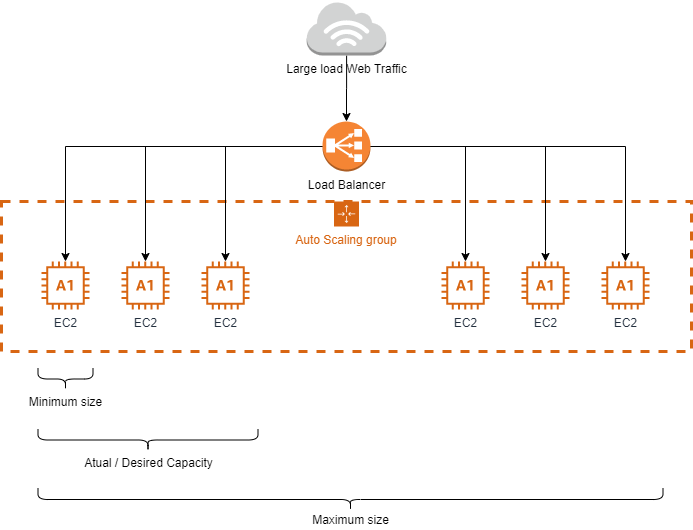
\includegraphics[scale=0.5]{elb_asg/elb_asg}
\centering\label{fig:elb_asg}
\end{figure}
